In this section I attempt to draw a clear picture about the semantic of the language. I speak about the anatomy of a visfile and a vismfile. I introduce some concepts and how the system should deal with them. Finally I explain how an indirection between the vismfile and the visfile is problematic in the context of a web-based environment and I attempt to draw the theoretical lines about a specific type of architecture to solve that problem. 


\begin{figure}
    \centering
    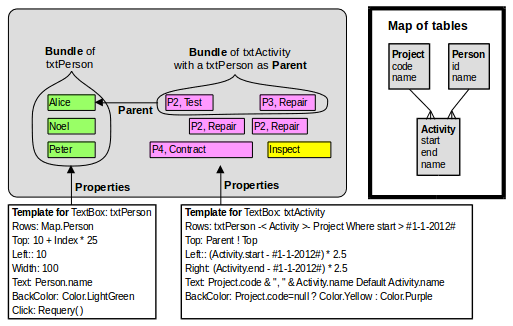
\includegraphics[width=0.9\textwidth]{images/uvisDiagram.png}
    \caption{uvis reference diagram found in the uvis card reference}
    \label{img:refDiagram}
\end{figure}

Throughout the rest of this report I recurrently refer to the reference diagram in figure~\ref{img:refDiagram}. It shows in a very concise manner the type of visualisations we are trying to achieve. The diagram is very minimal but it is subject to a very broad discussion.

\subsubsection{Anatomy of a Vis File}

\lstinputlisting[
    caption={example of a visfile},
    label={lst:visfileReference}
]{code/reference.vis}

A visfile is the textual specification of the components that must be rendered on the screen. Each component is described with a template which is represented in the visfile by the set of lines from the beginning of the file or from the previous template separator to the end of the file or to the next template separator. A template separator is characterized by two or more successive dash symbols (``--'').

Each template is made of properties that holds the necessary code (formula) for what should be evaluated and assigned to the properties of the different graphic instances that will ultimately be drawn on the screen. In the visfile, every line, except from template separators and commented lines (starting with the symbol~``\textquotesingle'') contains a template property. Each of them is a key-value pair representing the property name along with a formula. The formula is an expression that will typically be defined by the designer --with the eventual support of a ``drag-and-drop'' layer that the system should also provide-- and must be interpreted and evaluated by the visEngine.

Template properties can be separated into 3 distinct categories:
\begin{itemize}
    \item The first, mandatory, addresses the \emph{type} of Component to be instantiated and it's respective formula --which \emph{must} be a string-- gives its name to the template;
    \item The property with name Rows contains a formula that must be translated into a query string which will ultimately be sent against an external data service to retrieve the desired data resource instances. The construction of the query string depends on the in-memory ``query model'' that built by the system based on this formula;
    \item The rest of the properties in the template are providing formatting rules and behavioral rules for the resulting graphical controls. While evaluating the formulas for these properties, the resulting computed value will shadow\footnote{I refer here to the notion of ``variable shadowing''. The default value of a graphic control is not overwritten but rather masked behind the user-defined value. This is necessary because the user might decide to remove the declaration for the given property in the template. In this case the system should be able to retrieve the initial default value.} the default value defined in the targeted component.
\end{itemize}

When declaring a property in a template, the designer indirectly refer to a property of a component. It is possible for the system to determinate whether or not the declaration of a template property is legal by reflecting it's existence on the addressed component. Similarly, when assigning a value to a component property, the type of this value should be validated to ensure that it can be properly used, internally by the component (eg. when drawing the component).

The formula relating to a template's properties forms an expression tree. It's expressions have different types, either terminal or nonterminal lexical elements specified by the formal grammar they part of. A formula belongs to the family of context-free grammars which means that the evaluation of any nonterminal expression ultimately leads to the evaluation of a single terminal expression. An expression can have one of the following types:
\begin{itemize}
    \item \emph{identifiers}: Terminal expression whose value is a string which that can be used to uniquely address a resource in the system's runtime environment;
    \item \emph{numbers}: Terminal expression whose value is a number;
    \item \emph{strings}: Terminal expression whose value is a string;
    \item \emph{punctuations}: Terminal expression whose value is a punctuation symbol. eg: \texttt{!}, \texttt{.};
    \item \emph{operator}: Terminal expression whose value is an operator symbol or the string ``WHERE''. eg: \texttt{+}, \texttt{-}, \texttt{-<}, \texttt{WHERE};
    \item \emph{binary}: Nonterminal expression made of a left expression, an operator and a right expression. eg: \texttt{2~+~index~*~25};
    \item \emph{path}: Nonterminal expression made of an sequence alternating an identifier and a punctuation. The first element in the sequence can be either an identifier or a punctuation. eg: \texttt{Form.txtPerson}, \texttt{Map.activity.id}, \texttt{Parent!Top}, \texttt{!Me};
    \item \emph{formula}: Nonterminal expression working as a container for the entire expression tree.
\end{itemize}

In a formula, any operand can be a path. It allows the designer to walk into a specific address space\footnote{An Address space should be understood here in the sense of various objects accessible in the current environment (or scope) during the evaluation process} --enabling thereby the walk principle mentioned earlier-- in order to fetch some desired value. The punctuation value separating identifiers is used to either walk into a property of the component, when it is a bang symbol (``!'') or to walk into a data row when it is a dot symbol (``.''). Concretely, in the expression \texttt{Me.Top} the designer refers to the field with name Top in the data row of the current component whereas in the expression \texttt{Me!Top} he refers to the property with name Top of the current component. In principle, a path can have an undetermined length that matches the number of address spaces to walk into.

When an identifier in a path doesn't match any known object, the system should be able to infer if that identifier's value is a property of some object in the current scope and if so, use it's value. This allows the designer to omit to explicitly mention the address space. For instance, instead of typing Form.txtPerson he can simply type txtPerson in order to address the template with name txtPerson in the current form. If referring to more than a single object, the system should warn the designer that what he tries to address is ambiguous.

Parts of what the designer can address in the formula of a template property depends on what he defines in the Rows property. In listing~\ref{lst:visfileReference}, in the template named txtActivity, everything on the left hand-side of the ``WHERE'' operator indicate resources that must participate in the query that will be built for that particular template. In this case, two different types of objects are addressed: Another template in the current form (txtPerson) and two resources from the database (activity and project). When addressing a sibling template, the designer indirectly addresses the requested resource for that template, in this case: Map.person. The current template (txtActivity) becomes a child to the addressed template (txtPerson) and the entire query model gets written into the parent. In this case, that model should represent a request for all people, their related activities and for each activity the project it belongs to. What resource fields must participate in the query depends on what the designer addresses in the rest of the properties. For txtActivity, the field with name ``id'' in the resource with name ``activity'' and the field with name ``name'' in the resource with name ``project'' are candidate fields because they appear in the property of type ``Text''.

There is no guarantee in regards to the order in which a designer decides to declare the templates in the file. In order to determine if a template is the child or the parent of another one, a list of all existing templates must have been established beforehand. Listing~\ref{lst:visfileReference} shows the unfortunate case where a designer declared txtPerson after trying to address it in txtActivity. Without an existing list of all the declared templates in the file, this would cause the reference to point at an undeclared template.

Another unfortunate would occur if the designer addresses a template and from that template, refers back to the initial template. It would cause the system to infinitely look for the parent template causing a cyclic parent reference. This situation should be caught and prevented.

What clearly appears from studying the visfile is that the interpretation must be divided into two separate phases. A first phase, where the system builds the template and the query models and execute these models against the data provider (we will use the term pre-evaluate). A second phase where the system, based on the provided data instances will compute the actual expressions in the formulas (we will use the term evaluate).

Whether a relation made by designer between two different resources is valid can be verified thanks to a data map. The data map depends on the schema known by the data provider. Not all data-providers give the necessary informations about the relations between resources. VisTool relies on another type of file in order to properly build the data-map. It is also from this file that the system gets the information about what visfile should be opened on startup.

\subsubsection{Anatomy of a Vism File}
When an user wants a particular user-interface, he opens a vism file. This file holds the name of the vis file that contains the actual source code describing how the user-interface should look like. It also contains information about the database, what provider to use and how to access the data service. Moreover, the vism file is designed with the idea in mind that the local developer should be able to test the interfaces.

Through testing, one should be able to determine that all users easily understand how to read an interface, that abnormal data is shown properly (for instance if a requested dataset contains no data), that requests for external resources do not overload the service provider~\cite{lauesen2013}~p.13. 

\lstinputlisting[
    caption={example of a vismfile},
    label={lst:vismfileReference}
]{code/reference.vism}

Similarly as for the vis file, the vism file contains different blocks of code separated by the separator syntax ``--'' (I also use the term template to refer to those). Listing~\ref{lst:vismfileReference} shows how the maximal amount of external data resources to retrieve can be bound to an upper-limit. This ensures that no query will cause the system to block because it takes too long to compute. It also shows how the system's date can be manually defined in order to appropriately match a test scenario against the data to work with. When interacting with an interface an user can trigger update operations on the database. These updates can be simulated in which case the actual data in the database will not be affected.

The vism file makes it simple for the developer to switch from one database to another. Typically, when testing, multiple databases will be used to reflect different types of scenarios~\cite{lauesen2013}~p.13., the system takes this into account and allows to easily switch amongst them. This can be concretely done by adding a template to the file with a property with name Database and to address a specific provider (the system should have it's own set of built-in providers) along with a source as shown in listing~\ref{lst:vismfileReference}.

Finally, the file can also contain a description of the tables that should be made accessible through the system. When creating a table entry in the vismfile, it becomes addressable in the Rows property of the visfile. In addition to the name of the table an information can be given about how it relates to other tables that should also be registered in the file, of course.

In the local version of VisTool, an end-user opens a vism file just like he would in any other local program (like word or excel). The vismfile contains the name of the StartUpForm which describes the user interface that the system will generate when the file is opened. This interface is most likely made of components that helps to easily navigate to other vismfiles which in turn causes the system to open other visfiles and so on.
